\documentclass[article]{jss}
\usepackage{amsfonts,hyperref,enumerate}

%%%%%%%%%%%%%%%%%%%%%%%%%%%%%%
%% declarations for jss.cls %%
%%%%%%%%%%%%%%%%%%%%%%%%%%%%%%

%\usepackage{thumbpdf}

%% almost as usual
\author{David Meyer\\Wirtschaftsuniversit{\"a}t Wien \And
        Kurt Hornik\\Wirtschaftsuniversit{\"a}t Wien}
\title{Generalized and Customizable Sets in {\sf R}}

%% for pretty printing and a nice hypersummary also set:
\Plainauthor{David Meyer, Kurt Hornik} %% comma-separated

%% an abstract and keywords
\Abstract{
We present data structures and algorithms for
sets and some generalizations thereof (fuzzy
sets, multisets, and fuzzy multisets) available for {\sf R} through the
\pkg{sets} package. Fuzzy (multi-)sets are based on dynamically bound fuzzy
logic families. Further extensions include user-definable iterators
and matching functions.
}

\Keywords{\R, set, fuzzy logic, multiset, fuzzy set}
\Plainkeywords{R, sets, fuzzy logic, fuzzy set, multiset}

%\VignetteIndexEntry{Generalized and Customizable Sets in R}
%\VignetteDepends{sets,proxy}
%\VignetteKeywords{R, sets, fuzzy logic, fuzzy set, multiset}
%\VignettePackage{sets}

%% publication information
%% NOTE: This needs to filled out ONLY IF THE PAPER WAS ACCEPTED.
%% If it was not (yet) accepted, leave them commented.
%% \Volume{}
%% \Issue{}
%% \Month{May}
%% \Year{2009}
%% \Submitdate{2009-02-22}
%% \Acceptdate{2009-05-29}

%% The address of (at least) one author should be given
%% in the following format:
\Address{
  David Meyer\\
  Department of Information Systems and Operations\\
  E-mail: \email{David.Meyer@wu.ac.at}\\
  URL: \url{http://wi.wu.ac.at/~meyer/}\\

  Kurt Hornik\\
  Department of Statistics and Mathematics\\
  E-mail: \email{Kurt.Hornik@wu.ac.at}\\
  URL: \url{http://statmath.wu.ac.at/~hornik/}\\

  Wirtschaftsuniversit\"at Wien\\
  Augasse 2--6\\
  1090 Wien, Austria
}
%% It is also possible to add a telephone and fax number
%% before the e-mail in the following format:
%% Telephone: +43/1/31336-5053
%% Fax: +43/1/31336-734

%% for those who use Sweave please include the following line (with % symbols):
%% need no \usepackage{Sweave.sty}


\setkeys{Gin}{width=0.7\textwidth}


\newcommand\R{\textsf{R}}
\newcommand{\var}[1]{\textit{\texttt{#1}}}
\newcommand{\data}[1]{\texttt{#1}}
\newcommand{\class}[1]{\textsf{#1}}

\newcommand{\comment}[1]{\begin{quote} COMMENT. #1\end{quote}}

%% \code without `-' ligatures
\def\nohyphenation{\hyphenchar\font=-1 \aftergroup\restorehyphenation}
\def\restorehyphenation{\hyphenchar\font=`-}
{\catcode`\-=\active%
  \global\def\code{\bgroup%
    \catcode`\-=\active \let-\codedash%
    \Rd@code}}
\def\codedash{-\discretionary{}{}{}}
\def\Rd@code#1{\texttt{\nohyphenation#1}\egroup}

%% FIXME
\newcommand{\samp}[1]{\normalfont\texttt{#1}}

\newcommand{\eqn}[1]{$#1$}
\newcommand{\codefun}[1]{\code{#1()}}
\newcommand{\codefunind}[1]{\codefun{#1}\index{\texttt{#1}}}
\newcommand{\codeind}[1]{\code{#1}\index{\texttt{#1}}}
\newcommand{\sQuote}[1]{`{#1}'}
\newcommand{\dQuote}[1]{``{#1}''}

%% end of declarations %%%%%%%%%%%%%%%%%%%%%%%%%%%%%%%%%%%%%%%%%%%%%%%

\begin{document}

%% include your article here, just as usual
%% Note that you should use the \pkg{}, \proglang{} and \code{} commands.

\section[Introduction]{Introduction}

Only few will deny the importance of sets and set theory, building the
fundamentals of modern mathematics. For theory-building typically
axiomatic approaches \citep[e.g.,][]{sets:zermelo:1908, sets:fraenkel:1922}
are used. However, even
the primal, ``naive'' concept of sets representing ``collections
of distinct objects'' \citep{sets:cantor:1895} discarding order
and count information seems both natural and practical.
The main operation being ``is-element-of'', sets alone are of limited
\emph{practical} use---they most of the times serve as basic building blocks for
more complex structures such as relations and generalized sets. A
common way is to consider pairs $(X, m)$ with set $X$ (``universe'')
and membership function
$m : X \rightarrow D$ mapping each member to its ``grade''. The subset
of $X$ of elements with non-zero membership is called ``support''.
In \emph{multisets}, elements may appear more than once, i.e., $D =
\mathbb{N}_0$ ($m$ is also called the multiplicity function). There are many
applications in computer science and other disciplines
\citep[for a survey, see, e.g.,][]{sets:singh+ibrahim+yohanna:2007}.
In statistics, multisets appear as frequency tables. \emph{Fuzzy sets}
have become quite popular since their introduction by
\cite{sets:zadeh:1965}. Here, the membership function maps into the
unit interval. An interesting characteristic of fuzzy sets is that
the actual behavior of set operations depends on the underlying
fuzzy logic employed, which can be chosen according to domain-specific
needs. Fuzzy sets are actively used in fields such as machine
learning, engineering, medical science, and artificial intelligence
\citep{sets:dubois+prade+yager:1996}.
\emph{Fuzzy multisets} \citep{sets:yager:1986}
combine both approaches by allowing
each element to map to more than one fuzzy membership grade, i.e., $D$ is
the power set of multisets over the unit interval. Examples for the
application of fuzzy multisets can be found in the field of information
retrieval \citep[e.g.,][]{sets:matthe+caluwe+tre:2006}.

The use of sets and variants thereof is common in modern general purpose
programming languages:  \proglang{Java} and \proglang{C++}
provide corresponding abstract data types (ADTs) in their class
libraries, \proglang{Pascal} and \proglang{Python}
offer sets as native data type.
Indeed, since set elements are order-invariant and unique,
lookup mechanisms can be implemented very efficiently (for example via
hashing, resulting in nearly constant run-time complexity, compared to linear
search, requiring $n/2$ steps on the average for $n$ elements).
Surprisingly enough, sets are not standard in many
mathematical programming environments such as \proglang{Matlab} and
\proglang{Mathematica}, and also \R. Although the two latter offer
set operations such as union and intersection, these are applied to
linearly indexable structures (lists and vectors, respectively),
\emph{interpreting} them as sets. When it comes to \R,
this emulation is far from complete, and occasionally leads to inconsistent
behavior. First of all, the existing infrastructure has no clear concept
of how to compare elements, leading to possibly confusing
results when different data types are involved in
computations:
\begin{Schunk}
\begin{Sinput}
> s <- list(1, "1")
> union(s, s)
\end{Sinput}
\begin{Soutput}
[[1]]
[1] 1

[[2]]
[1] "1"
\end{Soutput}
\begin{Sinput}
> intersect(s, s)
\end{Sinput}
\begin{Soutput}
[[1]]
[1] 1
\end{Soutput}
\end{Schunk}
The reason is that most of the existing operations rely on
\codefun{match} which automatically performs type conversions
disturbing in this context.
Also, quite a few other basic operations such as
the Cartesian product, the power set, the subset predicate, etc., are
missing, let alone more specialized operations such as
the closure under union or intersection.
Then, the current facilities do not make use of a class
system, making extensions hard (if not impossible).  Another consequence
is that no distinction can be made between sequences (ordered
collections of objects) and sets (unordered collections of objects),
which is key for the definition of complex structures
where both concepts are combined such as relations.
Also, there is no support in base \R{} for extensions such as fuzzy sets
or multisets.

A few extension packages available from CRAN deal
with fuzzy concepts: Package \pkg{fuzzyFDR}
\citep{sets:lewin:2007}
calculates fuzzy decision rules for multiple testing, but does not
provide any explicit data structures for fuzzy sets.
The main functions in \pkg{fso}
\citep{sets:roberts:2007} for fuzzy set ordination compute and
return, among other information, membership values represented by
numeric matrices for some variables of the the input data.
\pkg{fuzzyRankTests} \citep{sets:geyer:2007} provides statistical tests
based on
fuzzy $p$ values and fuzzy confidence intervals, the latter being
returned as two separate numeric vectors for values and memberships. The
\pkg{gcl} package \citep{sets:vinterbo:2007}
infers fuzzy rules from the input data,
encapsulated in a classifying function returned by the training
function. The rules are composed of triangular fuzzy sets, represented
by triples describing the triangles' corner points for which the
memberships become $(0,1,0)$, respectively. Similarly, the \pkg{FKBL}
package for fuzzy knowledge base learning \citep{sets:alvarez:2007}
uses sequences of triangular fuzzy sets, defined by a vector of corner
points. Finally, \pkg{fuzzyOP} \citep{sets:aklan+altindas+macit:2008}
provides support for fuzzy
numbers: A set of $n$ numbers is represented by a $k \times 2n$
numeric matrix, where two consecutive columns represent (at most $k$)
supporting points and memberships,
respectively, of the corresponding piecewise linear
membership function. If some numbers have fewer supporting points than
others, the remaining cells are filled with missing values (\code{NA}s).

The \pkg{sets} package
\citep{sets:meyer+hornik:2008} presented here
provides a flexible and customizable basic infrastructure for
\emph{finite} sets and the generalizations mentioned above, including
basic operations for fuzzy logic. Apart from complementing the data
structures implemented in
base \R, extension packages like the ones mentioned above
could gain in flexibility from building on a common infrastructure,
facilitating data exchange and leveraging synergies.

The remainder of the paper is
structured as follows. In Section~\ref{sec:design}, we discuss the
design rationale of data structures and core algorithms.
Section~\ref{sec:sets} introduces the most important set
operations. Section~\ref{sec:gsets} starts with constructors and
specific methods for generalized sets, followed by a more focused
presentation of the fuzzy logic infrastructure, and of functionality for
handling and visualizing membership information. Section~\ref{sec:csets}
shows how generalized sets can further be customized by specifying
user-definable matching functions and
iterators.  Section~\ref{sec:examples} presents three examples before
Section~\ref{sec:conclusion} concludes.

\section{Design issues}
\label{sec:design}

There are many ways of implementing sets. Choice and efficiency largely
depend on the domain range (i.e., the number of possible values for each
element). If the domain is relatively small, i.e. in the range of integral
data types such as \code{byte}, \code{integer}, \code{word} etc., the
probably most efficient representation is an array of bits
representing the domain elements like in \proglang{Pascal}
\citep{sets:wirth:1983}.
Operations such as union and
intersection can then straightforwardly be implemented
using logical \code{OR} and \code{AND}, respectively.
This approach obviously fails for intractably large domains
(e.g., strings or recursive objects). Without
further application knowledge, one needs to resort to generic
container ADTs with efficient element access such as hash tables or
search trees (for unique elements).
Operations can then be implemented following the classical
element-based definitions: Union by
inserting all elements of the smaller set into the
larger one; intersection by creating a new set with
all elements of the smaller set also contained in the larger one;
etc.

Clearly, set comparison must be permutation invariant.
Some care is needed for nested sets. Assume, e.g., the comparison of
$A = \{1, \{2, 3\}\}$ and $B = \{1, \{3, 2\}\}$ which clearly are identical.
To implement set equality, a matching operator would be used to
check if all elements of $A$ are
contained in $B$. If elements were internally stored in this order during
creation, the objects representing
$\{2, 3\}$ and $\{3, 2\}$ would be different. Comparing two set elements
for equality would thus require to recursively compare all elements
down the nested structures, which can quickly become infeasible
computationally.
We avoid this by using a canonical ordering during set creation,
guaranteeing that identical sets have identical
physical representation as well. We chose to sort
elements using the natural order for numeric values, the
Unicode character representation for strings, and the serialization
byte sequence (as strings) for other objects.
Eventually, the ordered elements are stored in a list.

For the \pkg{sets} package, further limitations are imposed by the
extensions presented in Sections~\ref{sec:gsets} and
\ref{sec:csets}: Generalized sets require, for each element,
the membership information, and we also support user-defined, high-level
matching functions for comparing elements. Since operations defined
for generalized sets basically operate on the memberships,
it seems appropriate to store these as (generic) vectors in the same
order than the corresponding elements.
Thus, memberships of
separate sets can simply be combined element-wise.

Many operations (e.g., testing for equality, subsetting, intersection,
etc.) are based on matching elements of the sets involved.  This is
implemented by inserting the elements of the larger one into a hash
table (we use hashed environments), and to look up the elements of the
smaller set in this table \citep[p.~391]{sets:knuth:1973}.  As hash key,
we use the elements' character representation. Since different objects
might map to the same hash key, we actually store the \emph{indexes} of
the list elements, and match the actual objects using a simple linear
search. (Note that since the element list is sorted, elements with same
representation are grouped, so the search will typically be fast.)

The implementation is based on \R's \code{S3} class system, allowing
the definition of generic functions, dispatching appropriate methods
depending on the first argument's class information.
Objects for sets, generalized sets and customizable sets have
classes \class{set}, \class{gset} and \class{cset}, respectively, with
\class{set} inheriting from \class{gset} in turn inheriting from
\class{cset}.
Semantically suitable operators (such as \code{\&} for intersection)
are then overloaded to dispatch the right internal function
corresponding to the operands' classes.
Additionally, all operations can directly be accessed using the
corresponding name combined with a \samp{set\_}, \samp{gset\_}, or
\samp{cset\_} prefix to give the user
the choice of up- or downcasts when objects of different class levels
are involved in one computation. For example, consider the union of the
set $\{1\}$ and the fuzzy set $\{2/0.5\}$: using the generic operator
will give an error since the operands' classes differ. The user needs,
in fact, resolve the semantic ambiguity by explicitly choosing the
intended operation: If the result should be a
generalized (fuzzy) set, \codefun{gset\_union} should be used.  To make
the result a set (stripping membership information), s/he employs
\codefun{set\_union} instead.

\section{Sets}
\label{sec:sets}

The basic constructor for creating sets is the \codefunind{set}
function accepting any number of \R{}~objects as arguments.
\begin{Schunk}
\begin{Sinput}
> s <- set(1L, 2L, 3L)
> print(s)
\end{Sinput}
\begin{Soutput}
{1L, 2L, 3L}
\end{Soutput}
\end{Schunk}
For elements that are not sets or atomic vectors of length 1, the
print method for sets will use labels indicating the class (and
length for vectors):
\begin{Schunk}
\begin{Sinput}
> set("test", c, set("a", 2.5), list(1, 2))
\end{Sinput}
\begin{Soutput}
{"test", <<function>>, {"a", 2.5}, <<list(2)>>}
\end{Soutput}
\end{Schunk}
Mainly for cosmetic reasons, there is also a tuple class that can be
used for vectors:
\begin{Schunk}
\begin{Sinput}
> set(1, pair(1, 2), tuple(1L, 2L, 3L))
\end{Sinput}
\begin{Soutput}
{1, (1, 2), (1L, 2L, 3L)}
\end{Soutput}
\end{Schunk}
In addition, there is a generic \codefunind{as.set}
function coercing suitable objects to sets.
\begin{Schunk}
\begin{Sinput}
> s2 <- as.set(2:4)
> print(s2)
\end{Sinput}
\begin{Soutput}
{2L, 3L, 4L}
\end{Soutput}
\end{Schunk}
There are some basic predicate functions (and corresponding generic operators)
defined for the (in)equality (\code{!=}, \code{==}),
(proper) subset (\code{<}, \code{<=}), (proper) superset (\code{>},
\code{>=}), and element-of (\code{\%e\%}) operations:

\begin{Schunk}
\begin{Sinput}
> set_is_empty(set())
\end{Sinput}
\begin{Soutput}
[1] TRUE
\end{Soutput}
\begin{Sinput}
> set(1) <= set(1, 2)
\end{Sinput}
\begin{Soutput}
[1] TRUE
\end{Soutput}
\end{Schunk}
Note that all predicate functions are vectorized for convenience:
1:4 %e% set(1L, 2L, 3L)
The sequence \code{1:4} as \emph{one} element would be looked up by
using \code{list(1:4)} on the left-hand side.
The class-specific functions dispatched by the generic operators
are \codefun{set\_contains\_element},
\codefun{set\_is\_equal}, etc.
Other than these predicate functions, one can use
\codefun{length} for the cardinality:
\begin{Schunk}
\begin{Sinput}
> length(s)
\end{Sinput}
\begin{Soutput}
[1] 3
\end{Soutput}
\end{Schunk}
\codefun{c} and \code{|} for the union, \code{\&} for the intersection,
\code{\%D\%} for the symmetric difference:
\begin{Schunk}
\begin{Sinput}
> s | set("a")
\end{Sinput}
\begin{Soutput}
{"a", 1L, 2L, 3L}
\end{Soutput}
\begin{Sinput}
> s & s2
\end{Sinput}
\begin{Soutput}
{2L, 3L}
\end{Soutput}
\begin{Sinput}
> s %D% s2
\end{Sinput}
\begin{Soutput}
{1L, 4L}
\end{Soutput}
\end{Schunk}
\code{*} and \code{\^{ }$n$} for the ($n$-fold)
Cartesian product (yielding a set of $n$-tuples):
\begin{Schunk}
\begin{Sinput}
> s * s2
\end{Sinput}
\begin{Soutput}
{(1L, 2L), (1L, 3L), (1L, 4L), (2L, 2L), (2L, 3L), (2L, 4L), (3L, 2L),
 (3L, 3L), (3L, 4L)}
\end{Soutput}
\begin{Sinput}
> s^2L
\end{Sinput}
\begin{Soutput}
{(1L, 1L), (1L, 2L), (1L, 3L), (2L, 1L), (2L, 2L), (2L, 3L), (3L, 1L),
 (3L, 2L), (3L, 3L)}
\end{Soutput}
\end{Schunk}
and \code{2\^} for the power set:
\begin{Schunk}
\begin{Sinput}
> 2^s
\end{Sinput}
\begin{Soutput}
{{}, {1L}, {2L}, {3L}, {1L, 2L}, {1L, 3L}, {2L, 3L}, {1L, 2L, 3L}}
\end{Soutput}
\end{Schunk}
The class-specific functions
\codefunind{set\_union}, \codefunind{set\_intersection}, and
\codefunind{set\_symdiff} accept more than two arguments.\footnote{The
  $n$-ary symmetric difference of a collection of sets consists of all
  elements contained in an odd number of the sets in the collection.}
It is also possible to compute the \emph{relative} complement of a set $X$ in
$Y$, basically removing the elements of $X$ from $Y$:
\begin{Schunk}
\begin{Sinput}
> set_complement(set(1), set(1, 2, 3))
\end{Sinput}
\begin{Soutput}
{2, 3}
\end{Soutput}
\end{Schunk}
Note, however, that for sets (as opposed to \emph{generalized} sets),
the concept of a ``universe'' is not necessarily required, and
therefore the \emph{absolute} complement of a set not a well-defined operation.
In the \pkg{sets} package, objects of class
\class{set} are special cases of generalized sets. To stay faithful to
the simplicity of the original set concept,
we \emph{define} a \class{set} object's
universe to be identical to the set itself.
The \emph{absolute} complement of a \class{set} object
is therefore always the empty set:
\begin{Schunk}
\begin{Sinput}
> !set(1)
\end{Sinput}
\begin{Soutput}
{}
\end{Soutput}
\end{Schunk}

\codefunind{set\_combn} returns the set of all subsets of specified
length:
\begin{Schunk}
\begin{Sinput}
> set_combn(s, 2L)
\end{Sinput}
\begin{Soutput}
{{1L, 2L}, {1L, 3L}, {2L, 3L}}
\end{Soutput}
\end{Schunk}
\codefun{closure} and \codefun{reduction} compute the closure
and reduction under union or intersection for a set \emph{family}
(i.e., a set of sets):
\begin{Schunk}
\begin{Sinput}
> cl <- closure(set(set(1), set(2), set(3)), "union")
> print(cl)
\end{Sinput}
\begin{Soutput}
{{1}, {2}, {3}, {1, 2}, {1, 3}, {2, 3}, {1, 2, 3}}
\end{Soutput}
\begin{Sinput}
> reduction(cl, "union")
\end{Sinput}
\begin{Soutput}
{{1}, {2}, {3}}
\end{Soutput}
\end{Schunk}
The \codefun{Summary} group methods will also work if defined for the
elements:
\begin{Schunk}
\begin{Sinput}
> sum(s)
\end{Sinput}
\begin{Soutput}
[1] 6
\end{Soutput}
\begin{Sinput}
> range(s)
\end{Sinput}
\begin{Soutput}
[1] 1 3
\end{Soutput}
\end{Schunk}

Because set elements are unordered, it is not allowed to use positional
subscripting. However, sets can be subset and
elements be replaced by using the elements as index themselves:
\begin{Schunk}
\begin{Sinput}
> s2 <- set(1, 2, c, list(1, 2))
> print(s2)
\end{Sinput}
\begin{Soutput}
{<<function>>, 1, 2, <<list(2)>>}
\end{Soutput}
\begin{Sinput}
> s2[[c]] <- "foo"
> s2[[list(1, 2)]] <- "bar"
> print(s2)
\end{Sinput}
\begin{Soutput}
{"bar", "foo", 1, 2}
\end{Soutput}
\begin{Sinput}
> s2[list("foo", 1)]
\end{Sinput}
\begin{Soutput}
{"foo", 1}
\end{Soutput}
\end{Schunk}
Further, iterations over \emph{all}
elements can be carried out
using \codefun{for} and \codefun{lapply}/\codefun{sapply}:
\begin{Schunk}
\begin{Sinput}
> sapply(s, sqrt)
\end{Sinput}
\begin{Soutput}
[1] 1.000000 1.414214 1.732051
\end{Soutput}
\begin{Sinput}
> for (i in s) print(i)
\end{Sinput}
\begin{Soutput}
[1] 1
[1] 2
[1] 3
\end{Soutput}
\end{Schunk}
Note that \codefun{for} only
works because the underlying \proglang{C} code ignores
the class information, and directly
processes the low-level list representation instead. This will be
replaced by a more intelligent \dQuote{foreach} mechanism as soon as
it exists in base \R. \codefun{sapply} and \codefun{lapply} call the generic
\codefun{as.list} function before iterating over the elements. Since a
corresponding method exists for sets objects, this is
\dQuote{safer} than using \codefun{for}.

Using \codefunind{set\_outer},
it is possible to apply a function on all factorial combinations of the
elements of two sets.  If only one set is specified, the function is
applied on all pairs of this set.
\begin{Schunk}
\begin{Sinput}
> set_outer(set(1, 2), set(1, 2, 3), "/")
\end{Sinput}
\begin{Soutput}
  1   2         3
1 1 0.5 0.3333333
2 2 1.0 0.6666667
\end{Soutput}
\end{Schunk}
\section{Generalized sets}
\label{sec:gsets}

There are several extensions of sets such as \emph{fuzzy sets}
and \emph{multisets}. Both can be be seen as special cases of
\emph{fuzzy multisets}. All have in common that they are defined on some
\emph{universe} of elements, and that each element maps to some
membership information.
We present how generalized sets are constructed, and
demonstrate the effect of choosing different fuzzy logic families.

\subsection{Constructors and specific methods}

Generalized sets are created using the \codefun{gset} function. The
required arguments depend on whether membership information is specified
extensionally (listing members) or intensionally
(giving a rule for membership):

\begin{enumerate}
\item Extensional specification:
  \begin{enumerate}[a]
  \item Specify support and memberships as separate vectors. If
    memberships are omitted, they are assumed to be 1.
  \item Specify a set of elements along with their individual membership
    grades, using the element function (\codefun{e}).
  \end{enumerate}
\item Intensive specification: Specify universe and membership function.
\end{enumerate}

\noindent Note that for efficiency reasons, \codefun{gset} will not
store elements with zero memberships grades, and the specification of an
universe is only required with membership functions.
For convenience (and storage efficiency), a
default universe can be defined using \codefun{sets\_options}.
Set-specific universes supersede the default universe, if any.
If no universe (general or specific) is defined, the support of a set will be
interpreted as its universe. For multisets, the definition of a
(general or set-specific) universe can be complemented by a maximum
multiplicity or \emph{bound}.

\noindent Without membership information, \codefun{gset} creates a set (the support is converted to a set internally):
\begin{Schunk}
\begin{Sinput}
> X <- c("A", "B", "C")
> gset(support = X)
\end{Sinput}
\begin{Soutput}
{"A", "B", "C"}
\end{Soutput}
\end{Schunk}
Note, however, that unlike for \class{set} objects, it is possible to
define a universe that differs from (i.e., is a proper superset than)
the support:
\begin{Schunk}
\begin{Sinput}
> gset(support = X, universe = LETTERS[1:10])
\end{Sinput}
\begin{Soutput}
{"A", "B", "C"}
\end{Soutput}
\end{Schunk}
A multiset requires an integer membership vector:
\begin{Schunk}
\begin{Sinput}
> multi <- 1:3
> gset(support = X, memberships = multi)
\end{Sinput}
\begin{Soutput}
{"A" [1], "B" [2], "C" [3]}
\end{Soutput}
\end{Schunk}
For fuzzy sets, the memberships need to be out of the unit interval:
\begin{Schunk}
\begin{Sinput}
> ms <- c(0.1, 0.3, 1)
> gset(support = X, memberships = ms)
\end{Sinput}
\begin{Soutput}
{"A" [0.1], "B" [0.3], "C" [1]}
\end{Soutput}
\end{Schunk}
Alternatively to separate support / membership specification, each
elements can be paired with its membership value using \codefun{e}:
\begin{Schunk}
\begin{Sinput}
> gset(elements = list(e("A", 0.1), e("B", 0.2), e("C", 0.3)))
\end{Sinput}
\begin{Soutput}
{"A" [0.1], "B" [0.2], "C" [0.3]}
\end{Soutput}
\end{Schunk}
Fuzzy sets can, additionally, be created using a membership function,
applied to a specified (or the default) universe:
\begin{Schunk}
\begin{Sinput}
> f <- function(x) switch(x, A = 0.1, B = 0.2, C = 1, 0)
> gset(universe = X, charfun = f)
\end{Sinput}
\begin{Soutput}
{"A" [0.1], "B" [0.2], "C" [1]}
\end{Soutput}
\end{Schunk}
For fuzzy multisets,
the membership argument expects a list of membership grades,
either specified as vectors, or as multisets:
\begin{Schunk}
\begin{Sinput}
> ms2 <- list(c(0.1, 0.3, 0.4), c(1, 1), gset(support = ms, memberships = multi))
> gset(support = X, memberships = ms2)
\end{Sinput}
\begin{Soutput}
{"A" [{0.1, 0.3, 0.4}], "B" [{1 [2]}], "C" [{0.1 [1], 0.3 [2], 1 [3]}]}
\end{Soutput}
\end{Schunk}
\codefun{gset\_cardinality} returns the (relative) cardinality of a
generalized set, computed as the sum (mean) of all memberships.
\codefun{gset\_support}, \codefun{gset\_memberships}, \codefun{gset\_height}
and \codefun{gset\_core} can be used to retrieve support,
memberships, height (maximum membership degree),
and the core (elements with membership 1), respectively, of a
generalized set. \codefun{gset\_charfun} returns a (point-wise defined)
characteristic function for a given gset.
Note that in general, this will be different
from the characteristic function possibly used for the creation.

As for sets, the usual operations
such as union and intersection are available:
\begin{Schunk}
\begin{Sinput}
> X <- gset(c("A", "B", "C"), 4:6)
> Y <- gset(c("B", "C", "D"), 1:3)
> X | Y
\end{Sinput}
\begin{Soutput}
{"A" [4], "B" [5], "C" [6], "D" [3]}
\end{Soutput}
\begin{Sinput}
> X & Y
\end{Sinput}
\begin{Soutput}
{"B" [1], "C" [2]}
\end{Soutput}
\end{Schunk}
Additionally, the product (\codefun{gset\_product}), sum (\code{+}),
and difference (\code{-}) of sets are defined,
which multiply, add, and subtract
multiplicities (or memberships for fuzzy sets):
\begin{Schunk}
\begin{Sinput}
> X + Y
\end{Sinput}
\begin{Soutput}
{"A" [4], "B" [6], "C" [8], "D" [3]}
\end{Soutput}
\begin{Sinput}
> X - Y
\end{Sinput}
\begin{Soutput}
{"A" [4], "B" [4], "C" [4]}
\end{Soutput}
\begin{Sinput}
> gset_product(X, Y)
\end{Sinput}
\begin{Soutput}
{"B" [5], "C" [12]}
\end{Soutput}
\end{Schunk}
For fuzzy (multi-)sets, not only the relative, but also the
absolute complement (\code{!}) is defined:
\begin{Schunk}
\begin{Sinput}
> !gset(1, 0.3)
\end{Sinput}
\begin{Soutput}
{1 [0.7]}
\end{Soutput}
\begin{Sinput}
> X <- gset("a", universe = letters[1:3])
> !X
\end{Sinput}
\begin{Soutput}
{"b", "c"}
\end{Soutput}
\begin{Sinput}
> !(!X)
\end{Sinput}
\begin{Soutput}
{"a"}
\end{Soutput}
\begin{Sinput}
> !gset(1L, 2, universe = 1:3, bound = 3)
\end{Sinput}
\begin{Soutput}
{1L [1], 2L [3], 3L [3]}
\end{Soutput}
\end{Schunk}

\codefun{gset\_mean} creates a new set by averaging corresponding
memberships using the arithmetic, geometric or harmonic mean.
Note that missing elements have 0 membership degree:
\begin{Schunk}
\begin{Sinput}
> x <- gset(1:3, 1:3/3)
> y <- gset(1:2, 1:2/2)
> gset_mean(x, y)
\end{Sinput}
\begin{Soutput}
{1L [0.4166667], 2L [0.8333333], 3L [0.5]}
\end{Soutput}
\begin{Sinput}
> gset_mean(x, y, "harmonic")
\end{Sinput}
\begin{Soutput}
{1L [0.4], 2L [0.8]}
\end{Soutput}
\begin{Sinput}
> gset_mean(set(1), set(1, 2))
\end{Sinput}
\begin{Soutput}
{1 [1], 2 [0.5]}
\end{Soutput}
\end{Schunk}

The membership vector of a generalized set can be transformed via
\codefun{gset\_transform\_memberships}, applying any
\emph{vectorized} function to the memberships:
\begin{Schunk}
\begin{Sinput}
> x <- gset(1:10, 1:10/10)
> gset_transform_memberships(x, pmax, 0.5)
\end{Sinput}
\begin{Soutput}
{1L [0.5], 2L [0.5], 3L [0.5], 4L [0.5], 5L [0.5], 6L [0.6], 7L [0.7],
 8L [0.8], 9L [0.9], 10L [1]}
\end{Soutput}
\end{Schunk}
Note that for multisets, an element's
membership (multiplicity) $m$ is interpreted as a one-vector of length
$m$, yielding possibly unexpected results:
\begin{Schunk}
\begin{Sinput}
> x <- gset(1, 2)
> gset_transform_memberships(x, `*`, 0.5)
\end{Sinput}
\begin{Soutput}
{1 [{0.5 [2]}]}
\end{Soutput}
\end{Schunk}
For multisets, the \codefun{rep} function is a more natural choice
for membership transformations:
rep(x, 0.5)
In addition, three convenience functions are defined for fuzzy (multi-)sets:
\codefun{gset\_concentrate} and
\codefun{gset\_dilate} apply the square and the square root function,
and \codefun{gset\_normalize} normalizes the memberships to a specified
maximum:
\begin{Schunk}
\begin{Sinput}
> gset_dilate(y)
\end{Sinput}
\begin{Soutput}
{1L [0.7071068], 2L [1]}
\end{Soutput}
\begin{Sinput}
> gset_concentrate(y)
\end{Sinput}
\begin{Soutput}
{1L [0.25], 2L [1]}
\end{Soutput}
\begin{Sinput}
> gset_normalize(y, 0.5)
\end{Sinput}
\begin{Soutput}
{1L [0.25], 2L [0.5]}
\end{Soutput}
\end{Schunk}
(Note that these functions clearly have no effect for multisets.)

\subsection{Fuzzy logic and fuzzy sets}

For fuzzy (multi-)sets, the user can choose the logic underlying the
operations using the \codefun{fuzzy\_logic} function.  Fuzzy logics are
represented as named lists with four components \code{N}, \code{T},
\code{S}, and \code{I} containing the corresponding functions for
negation, conjunction (``t-norm''), disjunction (``t-conorm''), and
(residual) implication \citep{sets:klement+mesiar+pap:2000}.  The fuzzy
logic is selected by calling \codefun{fuzzy\_logic} with a character
string specifying the fuzzy logic ``family'', and optional
parameters. The exported functions \codefun{.N.}, \codefun{.T.},
\codefun{.S.}, and \codefun{.I.} reflect the currently selected
bindings. Available families include:  \code{"Zadeh"} (default),
\code{"drastic"}, \code{"product"}, \code{"Lukasiewicz"},
\code{"Fodor"}, \code{"Frank"}, \code{"Hamacher"},
\code{"Schweizer-Sklar"}, \code{"Yager"}, \code{"Dombi"},
\code{"Aczel-Alsina"}, \code{"Sugeno-Weber"}, \code{"Dubois-Prade"}, and
\code{"Yu"} (see Appendix \ref{sec:fuzzyfamilies}).  A call to
\codefun{fuzzy\_logic} without arguments returns the current logic.

\begin{Schunk}
\begin{Sinput}
> x <- 1:10/10
> y <- rev(x)
> .S.(x, y)
\end{Sinput}
\begin{Soutput}
 [1] 1.0 0.9 0.8 0.7 0.6 0.6 0.7 0.8 0.9 1.0
\end{Soutput}
\begin{Sinput}
> fuzzy_logic("Fodor")
> .S.(x, y)
\end{Sinput}
\begin{Soutput}
 [1] 1 1 1 1 1 1 1 1 1 1
\end{Soutput}
\end{Schunk}
Fuzzy set operations automatically use the active fuzzy logic setting:
\begin{Schunk}
\begin{Sinput}
> X <- gset(c("A", "B", "C"), c(0.3, 0.5, 0.8))
> print(X)
\end{Sinput}
\begin{Soutput}
{"A" [0.3], "B" [0.5], "C" [0.8]}
\end{Soutput}
\begin{Sinput}
> Y <- gset(c("B", "C", "D"), c(0.1, 0.3, 0.9))
> print(Y)
\end{Sinput}
\begin{Soutput}
{"B" [0.1], "C" [0.3], "D" [0.9]}
\end{Soutput}
\end{Schunk}
First, we try the Zadeh logic (default):
\begin{Schunk}
\begin{Sinput}
> fuzzy_logic("Zadeh")
> X & Y
\end{Sinput}
\begin{Soutput}
{"B" [0.1], "C" [0.3]}
\end{Soutput}
\begin{Sinput}
> X | Y
\end{Sinput}
\begin{Soutput}
{"A" [0.3], "B" [0.5], "C" [0.8], "D" [0.9]}
\end{Soutput}
\begin{Sinput}
> gset_complement(X, Y)
\end{Sinput}
\begin{Soutput}
{"B" [0.1], "C" [0.2]}
\end{Soutput}
\end{Schunk}
The results are different by switching to the Fodor logic:
\begin{Schunk}
\begin{Sinput}
> fuzzy_logic("Fodor")
> X & Y
\end{Sinput}
\begin{Soutput}
{"C" [0.3]}
\end{Soutput}
\begin{Sinput}
> X | Y
\end{Sinput}
\begin{Soutput}
{"A" [0.3], "B" [0.5], "C" [1], "D" [0.9]}
\end{Soutput}
\begin{Sinput}
> gset_complement(X, Y)
\end{Sinput}
\begin{Soutput}
{}
\end{Soutput}
\end{Schunk}
The \codefun{cut} method for generalized sets
\dQuote{filters} all elements with membership
not less then a specified level---the result, thus, is a crisp (multi)set:
\begin{Schunk}
\begin{Sinput}
> cut(X, 0.5)
\end{Sinput}
\begin{Soutput}
{"B", "C"}
\end{Soutput}
\end{Schunk}

\subsection{Characteristic functions and their visualization}
\label{sec:plots}

The \pkg{sets} package provides several generators of
characteristic functions to be used as templates for the creation of
fuzzy sets, including the following shapes:
gaussian curve (\codefun{fuzzy\_normal}),
double gaussian curve (\codefun{fuzzy\_two\_normals}),
bell curve (\codefun{fuzzy\_bell}),
sigmoid curve (\codefun{fuzzy\_sigmoid}),
PI curve (\codefun{fuzzy\_pi}),
trapezoid (\codefun{fuzzy\_trapezoid}),
and triangle (\codefun{fuzzy\_triangular}, \codefun{fuzzy\_cone}). For
example, a fuzzy normal function and a corresponding fuzzy set
are created using:
\begin{Schunk}
\begin{Sinput}
> N <- fuzzy_normal(mean = 0, sd = 1)
> N(-3:3)
\end{Sinput}
\begin{Soutput}
[1] 0.01110900 0.13533528 0.60653066 1.00000000 0.60653066 0.13533528 0.01110900
\end{Soutput}
\begin{Sinput}
> gset(charfun = N, universe = -3:3)
\end{Sinput}
\begin{Soutput}
{-3L [0.01110900], -2L [0.1353353], -1L [0.6065307], 0L [1], 1L
 [0.6065307], 2L [0.1353353], 3L [0.01110900]}
\end{Soutput}
\end{Schunk}
For convenience, we
also provide wrappers that directly generate corresponding sets,
given a specified universe:
\begin{Schunk}
\begin{Sinput}
> fuzzy_normal_gset(universe = -3:3)
\end{Sinput}
\begin{Soutput}
{-3L [0.01110900], -2L [0.1353353], -1L [0.6065307], 0L [1], 1L
 [0.6065307], 2L [0.1353353], 3L [0.01110900]}
\end{Soutput}
\end{Schunk}
(If no universe is specified, the default universe is used; if this is
also missing, the universe currently defaults to \code{seq(0, 20, 0.1)}.)
It is also possible to create function generators for characteristic
functions from other functions (such as distribution functions):
\begin{Schunk}
\begin{Sinput}
> fuzzy_poisson <- charfun_generator(dpois)
> gset(charfun = fuzzy_poisson(10), universe = seq(0, 20, 2))
\end{Sinput}
\begin{Soutput}
{0 [0.00036288], 2 [0.018144], 4 [0.1512], 6 [0.504], 8 [0.9], 10 [1],
 12 [0.7575758], 14 [0.4162504], 16 [0.1734377], 18 [0.05667898], 20
 [0.01491552]}
\end{Soutput}
\end{Schunk}
\codefun{fuzzy\_tuple} generates a sequence (tuple) of
sets based on any of the generating functions (except
\codefun{fuzzy\_trapezoid} and \codefun{fuzzy\_triangular}). The chosen
generating function is called with different
values (chosen along the universe) passed to the
first argument, thus varying the position or the resulting graph:
\begin{Schunk}
\begin{Sinput}
> fuzzy_tuple(fuzzy_normal, 5)
\end{Sinput}
\begin{Soutput}
(<<gset(201)>>, <<gset(201)>>, <<gset(201)>>, <<gset(201)>>,
 <<gset(201)>>)
\end{Soutput}
\end{Schunk}
(\verb|<<gset(201)>>| denotes an object of class \class{gset} with
201 elements---the size of the default universe).
The \pkg{sets} package provides support for visualizing the
membership functions of generalized
sets, and in particular fuzzy sets.
For (fuzzy) multisets, the plot method
produces a (grouped) barplot for
the membership vector (see Figure \ref{fig:plots}, top left):
\begin{Schunk}
\begin{Sinput}
> X <- gset(c("A", "B"), list(1:2/2, 0.5))
> plot(X)
\end{Sinput}
\end{Schunk}
Characteristic function generators can directly be plotted using a
default universe (see Figure \ref{fig:plots}, top right):
\begin{Schunk}
\begin{Sinput}
> plot(fuzzy_bell)
\end{Sinput}
\end{Schunk}
There is a plot method for tuples for visualizing a sequence
of sets (see Figure \ref{fig:plots}, bottom left):
\begin{Schunk}
\begin{Sinput}
> plot(fuzzy_tuple(fuzzy_cone, 10), col = gray.colors(10))
\end{Sinput}
\end{Schunk}
Plots of several sets can be superposed using the line method (see
Figure \ref{fig:plots}, bottom right):
\begin{Schunk}
\begin{Sinput}
> x <- fuzzy_normal_gset()
> y <- fuzzy_trapezoid_gset(corners = c(5, 10, 15, 17), height = c(0.7, 
+     1))
> plot(tuple(x, y), lty = 3)
> lines(x | y, col = 2)
> lines(gset_mean(x, y), col = 3, lty = 2)
\end{Sinput}
\end{Schunk}

\setkeys{Gin}{width=0.45\textwidth}
\begin{figure}[h]
\begin{center}
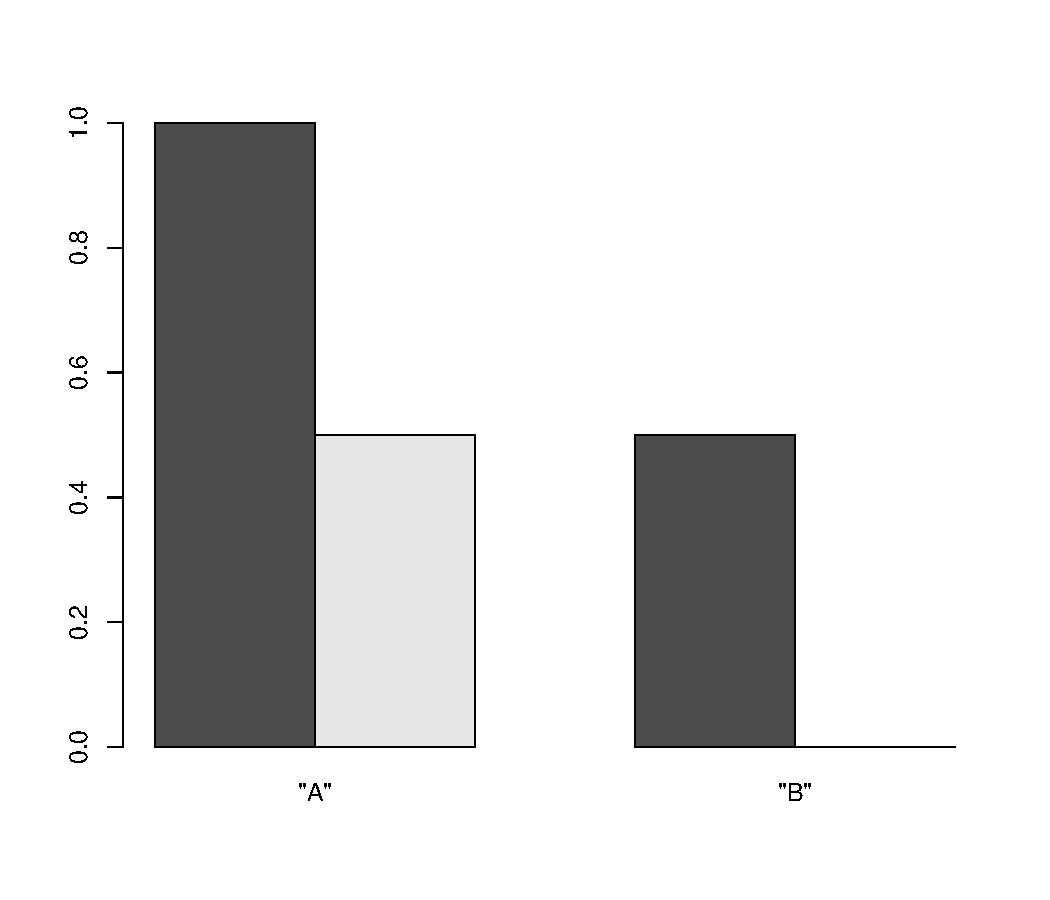
\includegraphics{JSS-plot1fig}
\hfill
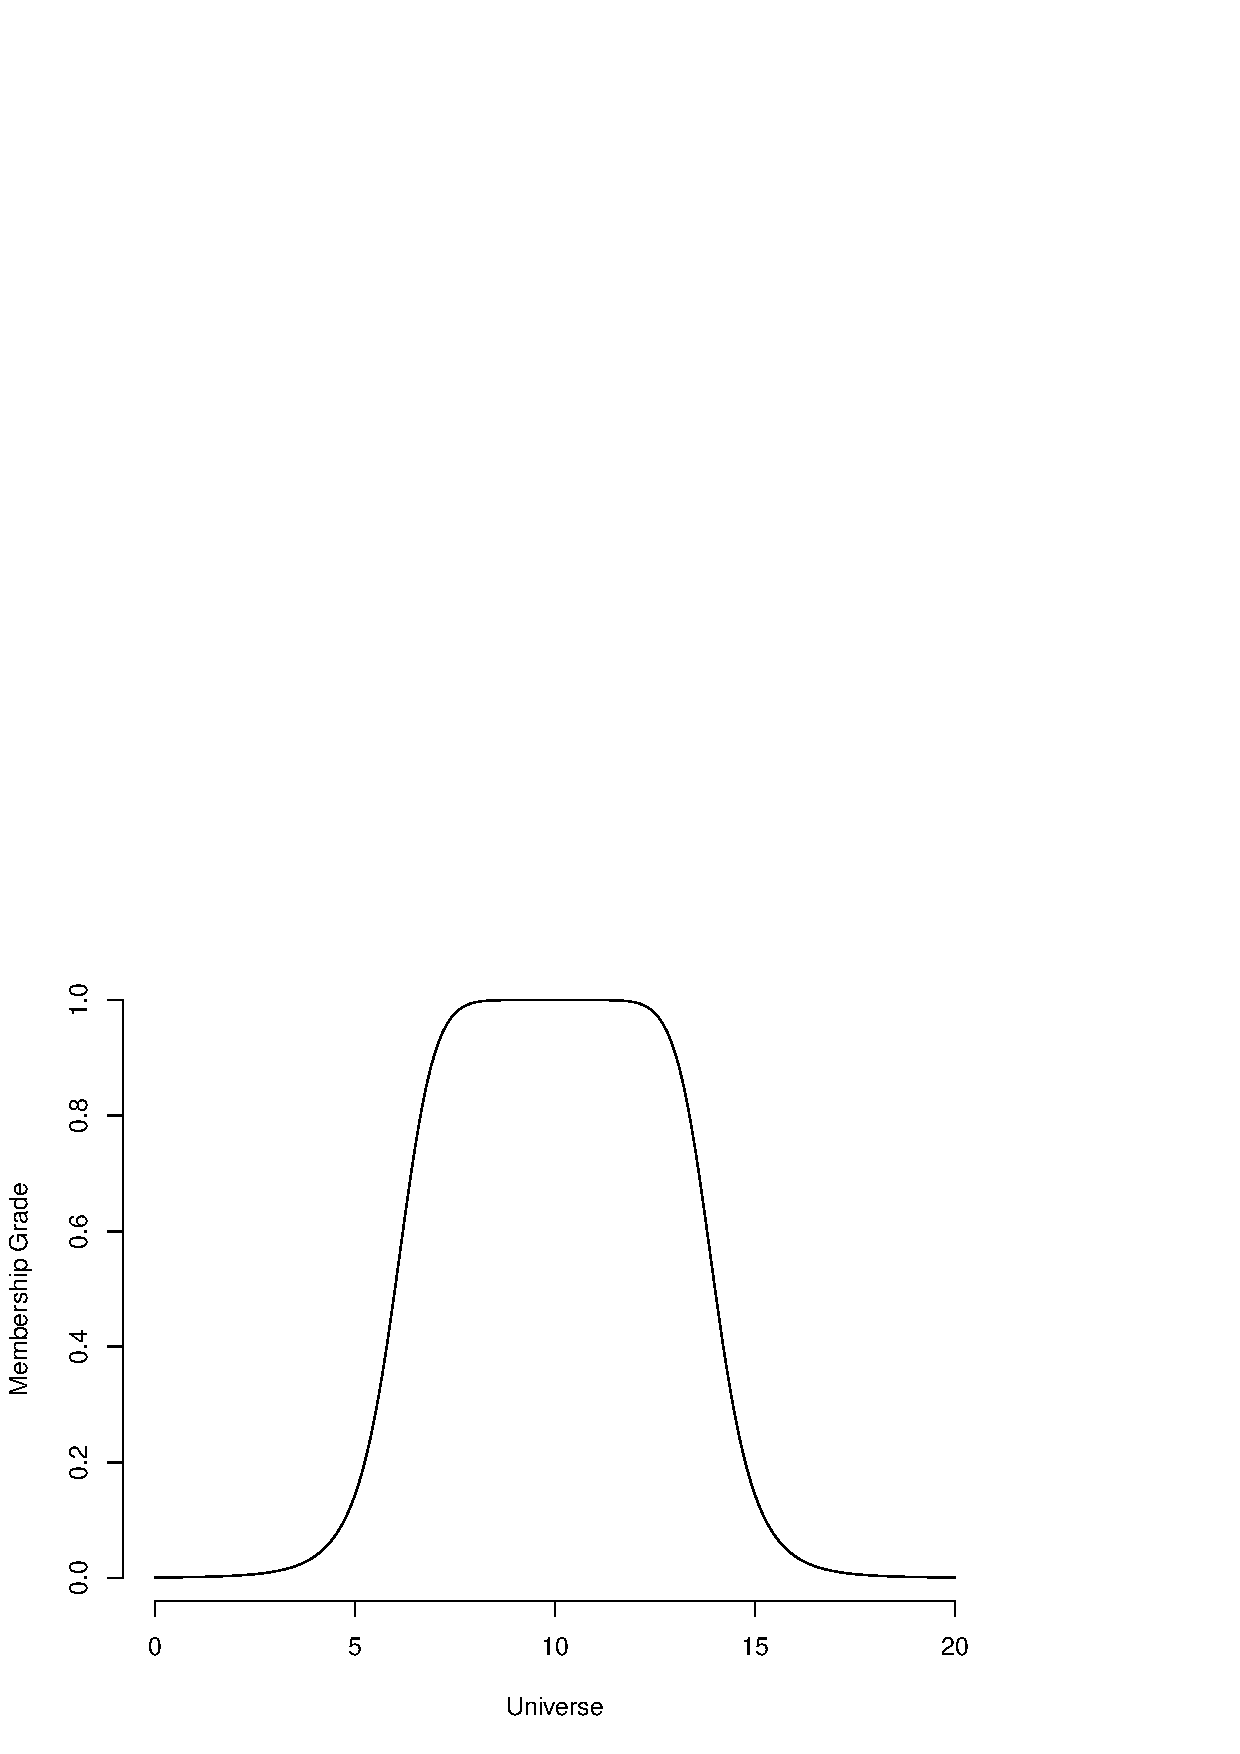
\includegraphics{JSS-plot2fig}
\hfill
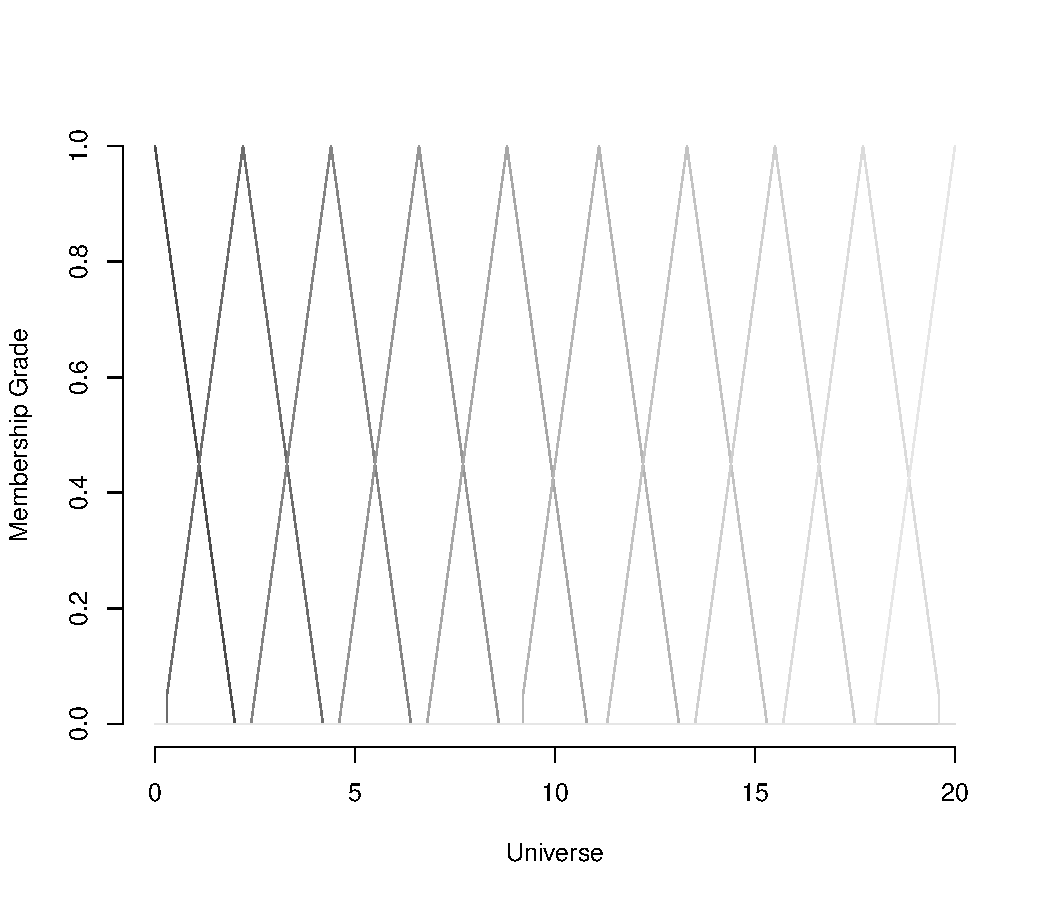
\includegraphics{JSS-plot3fig}
\hfill
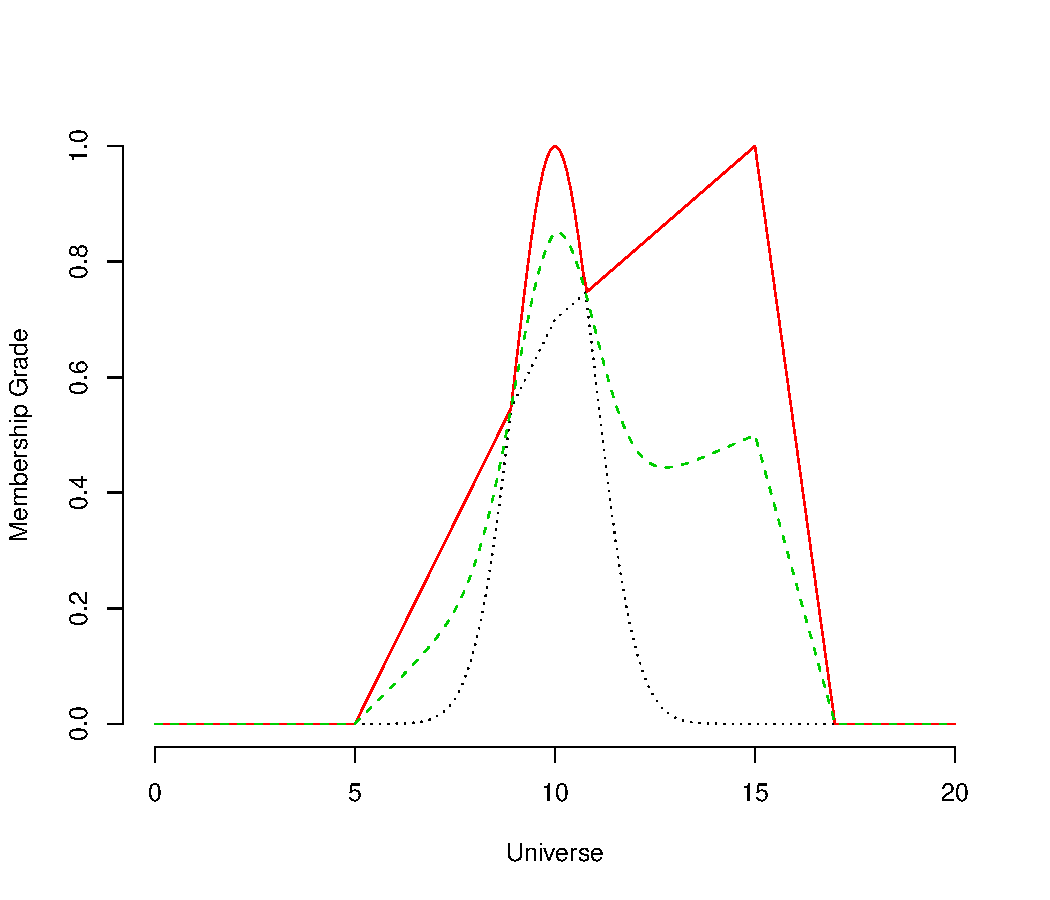
\includegraphics{JSS-plot4fig}
\caption{Membership plots for fuzzy sets. Top left: grouped barplot
  for a fuzzy multiset. Top right: graph of a bell curve. Bottom left:
sequence of triangular functions. Bottom right: two combinations of a
normal and a trapezoid function (dotted lines: basic shapes;
solid (red) line: union; dashed (green) line: arithmetic mean).}
\label{fig:plots}
\end{center}
\end{figure}

Finally, we note that the \pkg{sets} package provides basic
infrastructure for fuzzy inference (\codefun{fuzzy\_inference}),
involving the definition of
linguistic variables (\codefun{fuzzy\_variable}, \codefun{fuzzy\_partition})
and fuzzy rules (\codefun{fuzzy\_rule}) to build a fuzzy
system (\codefun{fuzzy\_system}). A few methods for defuzzification
(\codefun{gset\_defuzzify}) are also provided.

\section{User-definable extensions}
\label{sec:csets}

We added \emph{customizable sets}
extending generalized sets in two ways: First, users
can control the way elements are matched, i.e., define equivalence
classes of elements. Second, arbitrary iteration orders can be specified.

\subsection{Matching functions}

By default, sets and generalized sets use
\codefun{identical} to match elements which is maximally
restrictive. Note that this differs from the behavior of
\R's equality operator or
\codefun{match} which perform implicit type conversions
and thus confound, e.g., \code{1}, \code{1L} and \code{"1"}. In the
following example, note that on most computer systems, $3.3-2.2$ will not be
identical to $1.1$ due to numerical issues.
\begin{Schunk}
\begin{Sinput}
> x <- set("1", 1L, 1, 3.3 - 2.2, 1.1)
> print(x)
\end{Sinput}
\begin{Soutput}
{"1", 1L, 1, 1.1, 1.1}
\end{Soutput}
\begin{Sinput}
> y <- set(1, 1.1, 2L, "2")
> print(y)
\end{Sinput}
\begin{Soutput}
{"2", 2L, 1, 1.1}
\end{Soutput}
\begin{Sinput}
> 1L %e% y
\end{Sinput}
\begin{Soutput}
[1] FALSE
\end{Soutput}
\begin{Sinput}
> x | y
\end{Sinput}
\begin{Soutput}
{"1", "2", 1L, 2L, 1, 1.1, 1.1}
\end{Soutput}
\end{Schunk}
Customizable sets can be created using the \codefun{cset} constructor,
specifying the generalized set and some matching function.
\begin{Schunk}
\begin{Sinput}
> X <- cset(x, matchfun = match)
> print(X)
\end{Sinput}
\begin{Soutput}
{"1", 1.1}
\end{Soutput}
\begin{Sinput}
> Y <- cset(y, matchfun = match)
> print(Y)
\end{Sinput}
\begin{Soutput}
{"2", 1, 1.1}
\end{Soutput}
\begin{Sinput}
> 1L %e% Y
\end{Sinput}
\begin{Soutput}
[1] TRUE
\end{Soutput}
\begin{Sinput}
> X | Y
\end{Sinput}
\begin{Soutput}
{"1", "2", 1.1}
\end{Soutput}
\end{Schunk}
Matching functions take two
vector arguments, say, \code{x} and \code{table},
with \code{table} being a vector where the elements of \code{x} are looked up.
The function should be vectorized in the \code{x}, i.e. return the
first matching position for each element of \code{x}.
In order to make use of non-vectorized
predicates such as \codefun{all.equal}, the \pkg{sets} package
provides \codefun{matchfun} to generate one:
\begin{Schunk}
\begin{Sinput}
> FUN <- matchfun(function(x, y) isTRUE(all.equal(x, y)))
> X <- cset(x, matchfun = FUN)
> print(X)
\end{Sinput}
\begin{Soutput}
{"1", 1L, 1.1}
\end{Soutput}
\begin{Sinput}
> Y <- cset(y, matchfun = FUN)
> print(Y)
\end{Sinput}
\begin{Soutput}
{"2", 2L, 1, 1.1}
\end{Soutput}
\begin{Sinput}
> 1L %e% Y
\end{Sinput}
\begin{Soutput}
[1] TRUE
\end{Soutput}
\begin{Sinput}
> X | Y
\end{Sinput}
\begin{Soutput}
{"1", "2", 1L, 2L, 1.1}
\end{Soutput}
\end{Schunk}
\codefunind{sets\_options} can be used to conveniently switch the
default match and/or order function if a number of \class{cset} objects need
to be created:
\begin{Schunk}
\begin{Sinput}
> sets_options("matchfun", match)
> cset(x)
\end{Sinput}
\begin{Soutput}
{"1", 1.1}
\end{Soutput}
\begin{Sinput}
> cset(y)
\end{Sinput}
\begin{Soutput}
{"2", 1, 1.1}
\end{Soutput}
\begin{Sinput}
> cset(1:3) <= cset(c("1", "2", "3"))
\end{Sinput}
\begin{Soutput}
[1] FALSE
\end{Soutput}
\end{Schunk}

\subsection{Iterators}

In addition to specifying matching functions, it is possible to
change the order in which
iterators such as \codefun{as.list} (but not \codefun{for}---see end
of Section \ref{sec:sets})
process the elements. Note that the behavior of \codefun{as.list}
influences the labeling and print methods for
customizable sets. Sets and generalized sets
use the canonical internal ordering for iterations. With
customizable sets, a ``natural'' ordering of elements can be kept
by specifying either a permutation vector or an order function:

\begin{Schunk}
\begin{Sinput}
> cset(letters[1:5], orderfun = 5:1)
\end{Sinput}
\begin{Soutput}
{"e", "d", "c", "b", "a"}
\end{Soutput}
\begin{Sinput}
> FUN <- function(x) order(as.character(x), decreasing = TRUE)
> Z <- cset(letters[1:5], orderfun = FUN)
> print(Z)
\end{Sinput}
\begin{Soutput}
{"e", "d", "c", "b", "a"}
\end{Soutput}
\begin{Sinput}
> as.character(Z)
\end{Sinput}
\begin{Soutput}
[1] "e" "d" "c" "b" "a"
\end{Soutput}
\end{Schunk}
Note that converters for ordered factors keep the order:
\begin{Schunk}
\begin{Sinput}
> o <- ordered(c("a", "b", "a"), levels = c("b", "a"))
> as.set(o)
\end{Sinput}
\begin{Soutput}
{a, b}
\end{Soutput}
\begin{Sinput}
> as.gset(o)
\end{Sinput}
\begin{Soutput}
{a [2], b [1]}
\end{Soutput}
\begin{Sinput}
> as.cset(o)
\end{Sinput}
\begin{Soutput}
{b [1], a [2]}
\end{Soutput}
\end{Schunk}
Converters for other data types will use the order information
only if elements are unique:
\begin{Schunk}
\begin{Sinput}
> as.cset(c("A", "quick", "brown", "fox"))
\end{Sinput}
\begin{Soutput}
{"A", "quick", "brown", "fox"}
\end{Soutput}
\begin{Sinput}
> as.cset(c("A", "quick", "brown", "fox", "quick"))
\end{Sinput}
\begin{Soutput}
{"A" [1], "brown" [1], "fox" [1], "quick" [2]}
\end{Soutput}
\end{Schunk}

\section{Examples}
\label{sec:examples}

In the following, we present two examples for the use of multisets
and fuzzy multisets.

\subsection{Multisets}

Multisets are frequent in statistics since they can be seen as
frequency tables of some objects. Using the \pkg{sets} package, a
\dQuote{generalized} table can easily be constructed from a list of \R{}
objects using the \codefun{as.gset} coercion function. Assume, e.g., that one
samples a number of fourfold tables given the margins using \codefun{r2dtable}:
\begin{Schunk}
\begin{Sinput}
> set.seed(4711)
> l <- r2dtable(1000, r = 1:2, c = 2:1)
\end{Sinput}
\end{Schunk}
Since the sum of the first row (and second column) are constrained to
$1$, the top left cell entry can only be $0$ or $1$. Also, given the marginals,
there is only one degree of freedom in fourfold tables,
so the value of this first cell determines the others, and thus
only two possible tables exist:
\begin{Schunk}
\begin{Sinput}
> l[1:2]
\end{Sinput}
\begin{Soutput}
[[1]]
     [,1] [,2]
[1,]    0    1
[2,]    2    0

[[2]]
     [,1] [,2]
[1,]    1    0
[2,]    1    1
\end{Soutput}
\end{Schunk}
To count them, we can simply use \codefun{as.gset} that will construct a
multiset from the list:
\begin{Schunk}
\begin{Sinput}
> s <- as.gset(l)
> print(s)
\end{Sinput}
\begin{Soutput}
{<<2x2 matrix>> [330], <<2x2 matrix>> [670]}
\end{Soutput}
\end{Schunk}
Replace the matrices by the first cells' values:
\begin{Schunk}
\begin{Sinput}
> for (i in s) s[[i]] <- i[1]
> print(s)
\end{Sinput}
\begin{Soutput}
{0L [330], 1L [670]}
\end{Soutput}
\end{Schunk}
The estimated probabilities of having $0$ or $1$ in the first cell can thus
be obtained by:
\begin{Schunk}
\begin{Sinput}
> gset_memberships(s)/1000
\end{Sinput}
\begin{Soutput}
   1    2 
0.33 0.67 
\end{Soutput}
\end{Schunk}
The probability for $0$
clearly corresponds to the p value of the corresponding Fisher test:
\begin{Schunk}
\begin{Sinput}
> fisher.test(l[[1]])$p.value
\end{Sinput}
\begin{Soutput}
[1] 0.3333333
\end{Soutput}
\end{Schunk}

\subsection{Fuzzy multisets}

Fuzzy multisets can be used to represent objects appearing several
times with different membership grades (e.g., weights, degrees of
credibility, \dots). \cite{sets:mizutani+inokuchi+miyamoto:2008}
describe an interesting application of fuzzy multisets to text mining:
The occurrences of some terms of interest (``neural network'',
``fuzzy'', ``image'') in titles, abstracts, and keywords
of 30 documents on fuzzy theory are represented by fuzzy
multisets, with varying memberships depending on whether a term occurs
in the title (degree 1), the keywords (degree 0.6), and/or the
abstract (degree 0.2).
\begin{Schunk}
\begin{Sinput}
> data("fuzzy_docs")
> print(fuzzy_docs[8:9])
\end{Sinput}
\begin{Soutput}
$x8
{"fuzzy" [{0.2, 0.6}], "neural network" [{0.2, 1}]}

$x9
{"fuzzy" [{0.2, 0.6, 1}], "image" [{0.6}], "neural network" [{0.2, 0.6,
 1}]}
\end{Soutput}
\end{Schunk}
This information is then used to compute distances between documents,
and ultimately to compare several (non-linear) clustering methods
regarding their abilities of recovering the true underlying
structure. In fact, it is known that the first 12 documents are
related to neural networks, and the remaining 18 to image
processing.

In the following, we will perform simple hierarchical
clustering. We start by computing a distance matrix for the 30
documents. The \pkg{sets} package implements the
Jaccard dissimilarity, defined as
$1 - |X \cap Y| / |X \cup Y|$ given two generalized sets $X$ and $Y$, $|\cdot|$
denoting the cardinality for generalized sets.
A corresponding dissimilarity matrix can be obtained using,
e.g., the \pkg{proxy} package \citep{sets:meyer+buchta:2008}:
\begin{Schunk}
\begin{Sinput}
> library(proxy)
> d <- dist(fuzzy_docs, gset_dissimilarity)
\end{Sinput}
\end{Schunk}
We then apply Ward's clustering method:
\begin{Schunk}
\begin{Sinput}
> cl1 <- hclust(d, "ward")
\end{Sinput}
\end{Schunk}
resulting in a clustering depicted in Figure \ref{fig:cluster1}.
Clearly, the neural network-related documents (\#1--\#12) are separated from
the image processing papers:
\begin{Schunk}
\begin{Sinput}
> labs1 <- cutree(cl1, 2)
> print(labs1)
\end{Sinput}
\begin{Soutput}
 x1  x2  x3  x4  x5  x6  x7  x8  x9 x10 x11 x12 x13 x14 x15 x16 x17 x18 x19 x20 
  1   1   1   1   1   1   1   1   1   1   1   1   2   2   2   2   2   2   2   2 
x21 x22 x23 x24 x25 x26 x27 x28 x29 x30 
  2   2   2   2   2   2   2   2   2   2 
\end{Soutput}
\end{Schunk}

\setkeys{Gin}{width=0.7\textwidth}
\begin{figure}[h]
\begin{center}
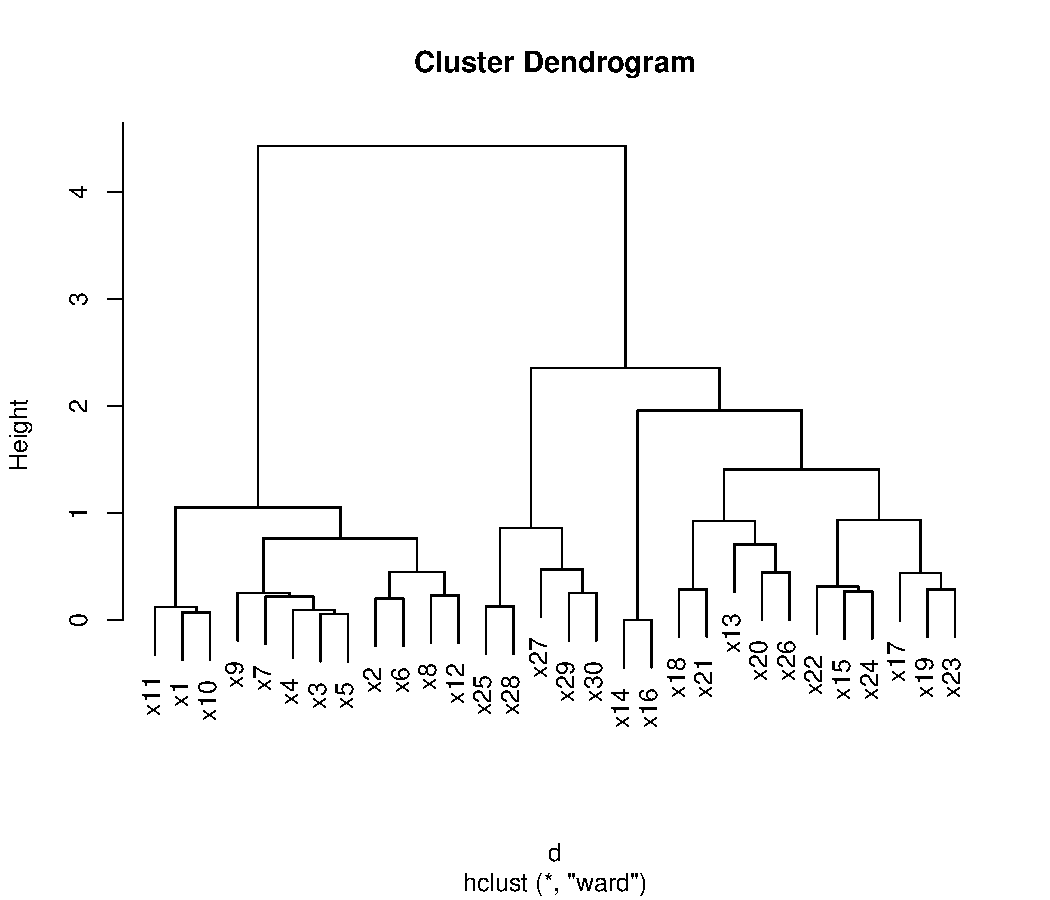
\includegraphics{JSS-clusterplot}
\caption{Dendrogram for the \texttt{fuzzy\_docs} data, clustered using
  Ward's method on Jaccard distances computed from fuzzy multisets.}
\label{fig:cluster1}
\end{center}
\end{figure}

Note that for this data, using
different weightings for terms in titles, keywords and
abstracts are key to recover the subgroups.
Naive text mining approaches operate on ``classical''
term-document-matrices only, counting term occurrences without further
information on their relevance:
\begin{Schunk}
\begin{Sinput}
> tdm <- set_outer(c("neural networks", "fuzzy", "image"), fuzzy_docs, 
+     `%in%`)
> print(tdm)
\end{Sinput}
\begin{Soutput}
                   x1    x2    x3    x4    x5    x6    x7    x8    x9   x10
neural networks FALSE FALSE FALSE FALSE FALSE FALSE FALSE FALSE FALSE FALSE
fuzzy            TRUE  TRUE  TRUE  TRUE  TRUE  TRUE  TRUE  TRUE  TRUE  TRUE
image           FALSE FALSE FALSE FALSE FALSE FALSE FALSE FALSE  TRUE  TRUE
                  x11   x12   x13   x14   x15   x16   x17   x18   x19   x20
neural networks FALSE FALSE FALSE FALSE FALSE FALSE FALSE FALSE FALSE FALSE
fuzzy            TRUE  TRUE  TRUE FALSE  TRUE FALSE  TRUE  TRUE FALSE  TRUE
image            TRUE  TRUE  TRUE  TRUE  TRUE  TRUE  TRUE  TRUE  TRUE  TRUE
                  x21   x22   x23   x24   x25   x26   x27   x28   x29   x30
neural networks FALSE FALSE FALSE FALSE FALSE FALSE FALSE FALSE FALSE FALSE
fuzzy            TRUE  TRUE  TRUE  TRUE  TRUE  TRUE FALSE FALSE FALSE FALSE
image            TRUE  TRUE  TRUE  TRUE  TRUE  TRUE  TRUE  TRUE  TRUE  TRUE
\end{Soutput}
\end{Schunk}
By again computing Jaccard distances:
\begin{Schunk}
\begin{Sinput}
> d <- dist(tdm, "Jaccard", by_rows = FALSE)
\end{Sinput}
\end{Schunk}
and the corresponding hierarchical clustering,
visualized in Figure \ref{fig:cluster2}:
\begin{Schunk}
\begin{Sinput}
> cl2 <- hclust(d, "ward")
\end{Sinput}
\end{Schunk}
we can see that the ``standard'' text mining approach fails to
correctly assign four documents (\#9--\#12):
\begin{Schunk}
\begin{Sinput}
> labs2 <- cutree(cl2, 2)
> print(labs2)
\end{Sinput}
\begin{Soutput}
 x1  x2  x3  x4  x5  x6  x7  x8  x9 x10 x11 x12 x13 x14 x15 x16 x17 x18 x19 x20 
  1   1   1   1   1   1   1   1   2   2   2   2   2   2   2   2   2   2   2   2 
x21 x22 x23 x24 x25 x26 x27 x28 x29 x30 
  2   2   2   2   2   2   2   2   2   2 
\end{Soutput}
\begin{Sinput}
> table(labs1, labs2)
\end{Sinput}
\begin{Soutput}
     labs2
labs1  1  2
    1  8  4
    2  0 18
\end{Soutput}
\end{Schunk}

\setkeys{Gin}{width=0.7\textwidth}
\begin{figure}[h]
\begin{center}
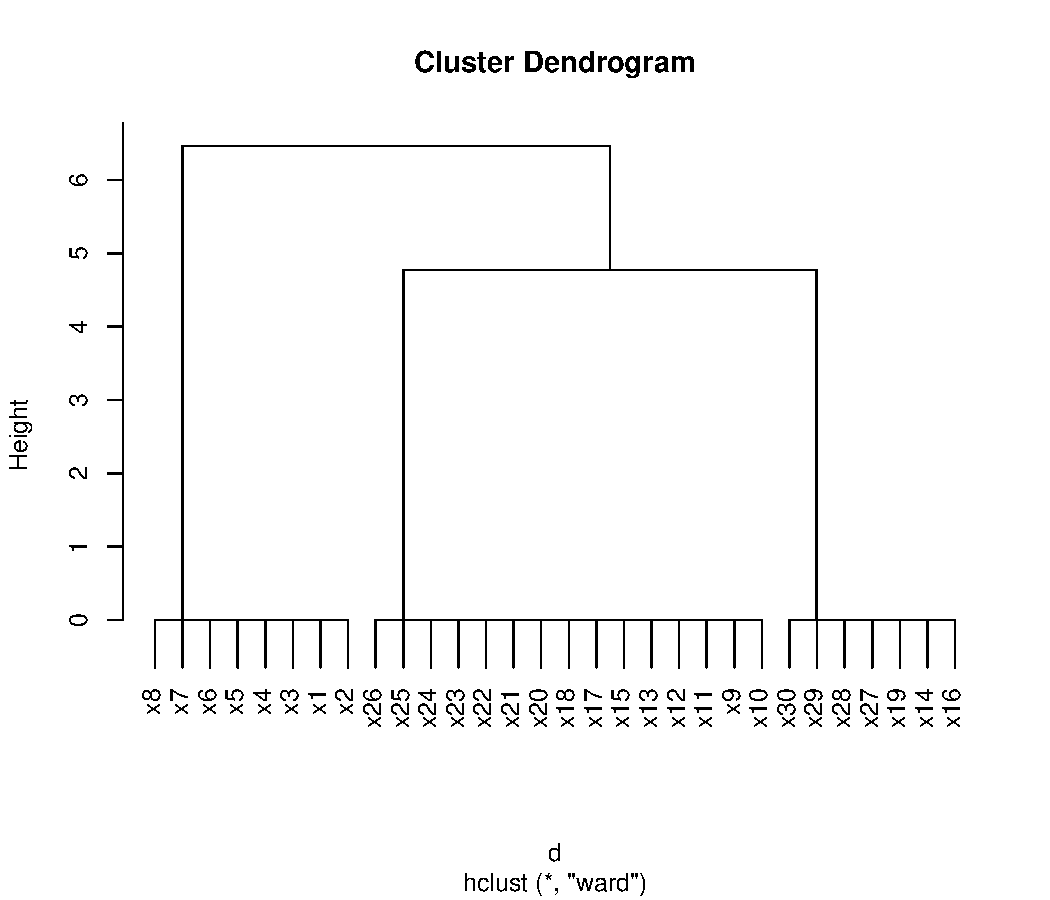
\includegraphics{JSS-clusterplot2}
\caption{Dendrogram for the \texttt{fuzzy\_docs} data, using Ward's
  method on a term-document-matrix generated for the data.}
\label{fig:cluster2}
\end{center}
\end{figure}

\section{Conclusion}
\label{sec:conclusion}

In this paper, we described the \pkg{sets} package for \R, providing
infrastructure for sets and generalizations thereof such as fuzzy
sets, multisets and fuzzy multisets. The fuzzy variants make use of a
dynamic fuzzy logic infrastructure offering several fuzzy logic
families. Generalized sets are further extended to allow for
user-defined iterators and matching functions. Current work focuses on
data structures and algorithms for relations,
an important application of sets.

\begin{appendix}

\section{Available fuzzy logic families}
\label{sec:fuzzyfamilies}

  Let us
  refer to \eqn{N(x) = 1 - x} as the \emph{standard} negation, and,
  for a t-norm \eqn{T}, let \eqn{S(x, y) = 1 - T(1 - x, 1 - y)} be the
  \emph{dual} (or complementary) t-conorm.  Available specifications and
  corresponding families are as follows, with the standard negation used
  unless stated otherwise.

  \begin{description}
    \item[\code{"Zadeh"}]{Zadeh's logic with \eqn{T = \min} and
      \eqn{S = \max}.  Note that the minimum t-norm, also known as the
      G{\"o}del t-norm, is the pointwise largest t-norm, and that the
      maximum t-conorm is the smallest t-conorm.}
    \item[\code{"drastic"}]{the drastic logic with t-norm
      \eqn{T(x, y) = y} if \eqn{x = 1}, \eqn{x} if \eqn{y = 1}, and 0
      otherwise, and complementary t-conorm \eqn{S(x, y) = y} if
      \eqn{x = 0}, \eqn{x} if \eqn{y = 0}, and 1 otherwise.  Note that
      the drastic t-norm and t-conorm are the smallest t-norm and
      largest t-conorm, respectively.}
    \item[\code{"product"}]{the family with the product t-norm
      \eqn{T(x, y) = xy} and dual t-conorm \eqn{S(x, y) = x + y - xy}.}
    \item[\code{"Lukasiewicz"}]{the \L{}ukasiewicz logic with t-norm
      \eqn{T(x, y) = \max(0, x + y - 1)} and dual t-conorm
      \eqn{S(x, y) = \min(x + y, 1)}.}
    \item[\code{"Fodor"}]{the family with Fodor's \emph{nilpotent
	minimum} t-norm given by \eqn{T(x, y) = \min(x, y)} if
      \eqn{x + y > 1}, and 0 otherwise, and the dual t-conorm given by
    \eqn{S(x, y) = \max(x, y)} if \eqn{x + y < 1}, and 1 otherwise.}
    \item[\code{"Frank"}]{the family of Frank t-norms \eqn{T_p},
      \eqn{p \ge 0}, which gives the Zadeh, product and \L{}ukasiewicz
      t-norms for \eqn{p = 0}, 1, and \eqn{\infty}, respectively,
      and otherwise is given by
      \eqn{T(x, y) = \log_p (1 + (p^x - 1) (p^y - 1) / (p - 1))}.}
    \item[\code{"Hamacher"}]{the three-parameter family of Hamacher,
      with negation \eqn{N_\gamma(x) = (1 - x) / (1 + \gamma x)},
      t-norm  \eqn{T_\alpha(x, y) = xy / (\alpha + (1 - \alpha)(x + y - xy))},
      and t-conorm
      \eqn{S_\beta(x, y) = (x + y + (\beta - 1) xy) / (1 + \beta xy)},
      where \eqn{\alpha \ge 0} and \eqn{\beta, \gamma \ge -1}.  This
      gives a deMorgan triple (for which $N(S(x, y)) = T(N(x), N(y))$
      iff \eqn{\alpha = (1 + \beta) / (1 + \gamma)}.}
  \end{description}

  \noindent The following parametric families are obtained by combining the
  corresponding families of t-norms with the standard negation and
  complementary t-conorm.

  \begin{description}
  \item[\code{"Schweizer-Sklar"}]{the Schweizer-Sklar family
      \eqn{T_p}, \eqn{-\infty \le p \le \infty}, which
      gives the Zadeh (minimum), product and drastic t-norms for
      \eqn{p = -\infty}, \eqn{0}, and \eqn{\infty},
      respectively, and otherwise is given by
      \eqn{T_p(x, y) = \max(0, (x^p + y^p - 1)^{1/p})}.}
  \item[\code{"Yager"}]{the Yager family \eqn{T_p}, \eqn{p \ge 0},
      which gives the drastic and minimum t-norms for \eqn{p = 0}
      and \eqn{\infty}, respectively, and otherwise is given by
      \eqn{T_p(x, y) = \max(0, 1 - ((1-x)^p + (1-y)^p)^{1/p})}.}
  \item[\code{"Dombi"}]{the Dombi family \eqn{T_p}, \eqn{p \ge 0},
      which gives the drastic and minimum t-norms for \eqn{p = 0}
      and \eqn{\infty}, respectively, and otherwise is given by
      \eqn{T_p(x, y) = 0} if \eqn{x = 0} or \eqn{y = 0}, and
      \eqn{T_p(x, y) = 1 / (1 + ((1/x - 1)^p + (1/y - 1)^p)^{1/p})} if
      both \eqn{x > 0} and \eqn{y > 0}.}
  \item[\code{"Aczel-Alsina"}]{the family of t-norms \eqn{T_p},
      \eqn{p \ge 0}, introduced by Acz{\'e}l and Alsina, which gives the
      drastic and minimum t-norms for \eqn{p = 0} and
      \eqn{\infty}, respectively, and otherwise is given by
      \eqn{T_p(x, y) = \exp(-(|\log(x)|^p + |\log(y)|^p)^{1/p})}.}
  \item[\code{"Sugeno-Weber"}]{the family of t-norms \eqn{T_p},
      \eqn{-1 \le p \le \infty}, introduced by Weber
      with dual t-conorms introduced by Sugeno, which gives the
      drastic and product t-norms for \eqn{p = -1} and
      \eqn{\infty}, respectively, and otherwise is given by
      \eqn{T_p(x, y) = \max(0, (x + y - 1 + pxy) / (1 + p))}.}
  \item[\code{"Dubois-Prade"}]{the family of t-norms \eqn{T_p},
      \eqn{0 \le p \le 1}, introduced by Dubois and Prade, which gives
      the minimum and product t-norms for \eqn{p = 0} and \eqn{1},
      respectively, and otherwise is given by
      \eqn{T_p(x, y) = xy / \max(x, y, p)}.}
  \item[\code{"Yu"}]{the family of t-norms \eqn{T_p}, \eqn{p \ge -1},
      introduced by Yu, which gives the product and drastic t-norms for
      \eqn{p = -1} and \eqn{\infty}, respectively, and otherwise is
      given by \eqn{T(x, y) = \max(0, (1 + p) (x + y - 1) - p x y)}.}
  \end{description}

\end{appendix}

\bibliography{sets}

\end{document}
